
\chapter{Mach waves, shock waves and Prandtl-Meyer expansion}
\section{Weak solutions of the flow equations}
	Flow equations also allow non-continuous solutions $\rightarrow$ \textbf{weak}. We limit the study to stationary weak solutions for which the discontinuity does not change in time. We restrict ourselves to non viscous 2D flows, respecting Euler equations (mass, momentum, energy) which allows discontinuities. Let's remind the Euler hyperbolic equation and the scalar convection equation: 
	
	\begin{equation}
	\frac{\D u}{\D t} + a \frac{\D u}{\D x} = 0 \qquad u = f(x-at) = f(q)
	\end{equation}
	
	The derivatives give: 
	
	\begin{equation}
	\frac{\D u}{\D t} = \frac{\D f}{\D q} \frac{\D q}{\D t} = \frac{\D f}{\D q} (-a)\qquad \frac{\D u}{\D x} = \frac{\D f}{\D q} \frac{\D q}{\D x} = \frac{\D f}{\D q} (1)
	\end{equation}
	
	\begin{center}
	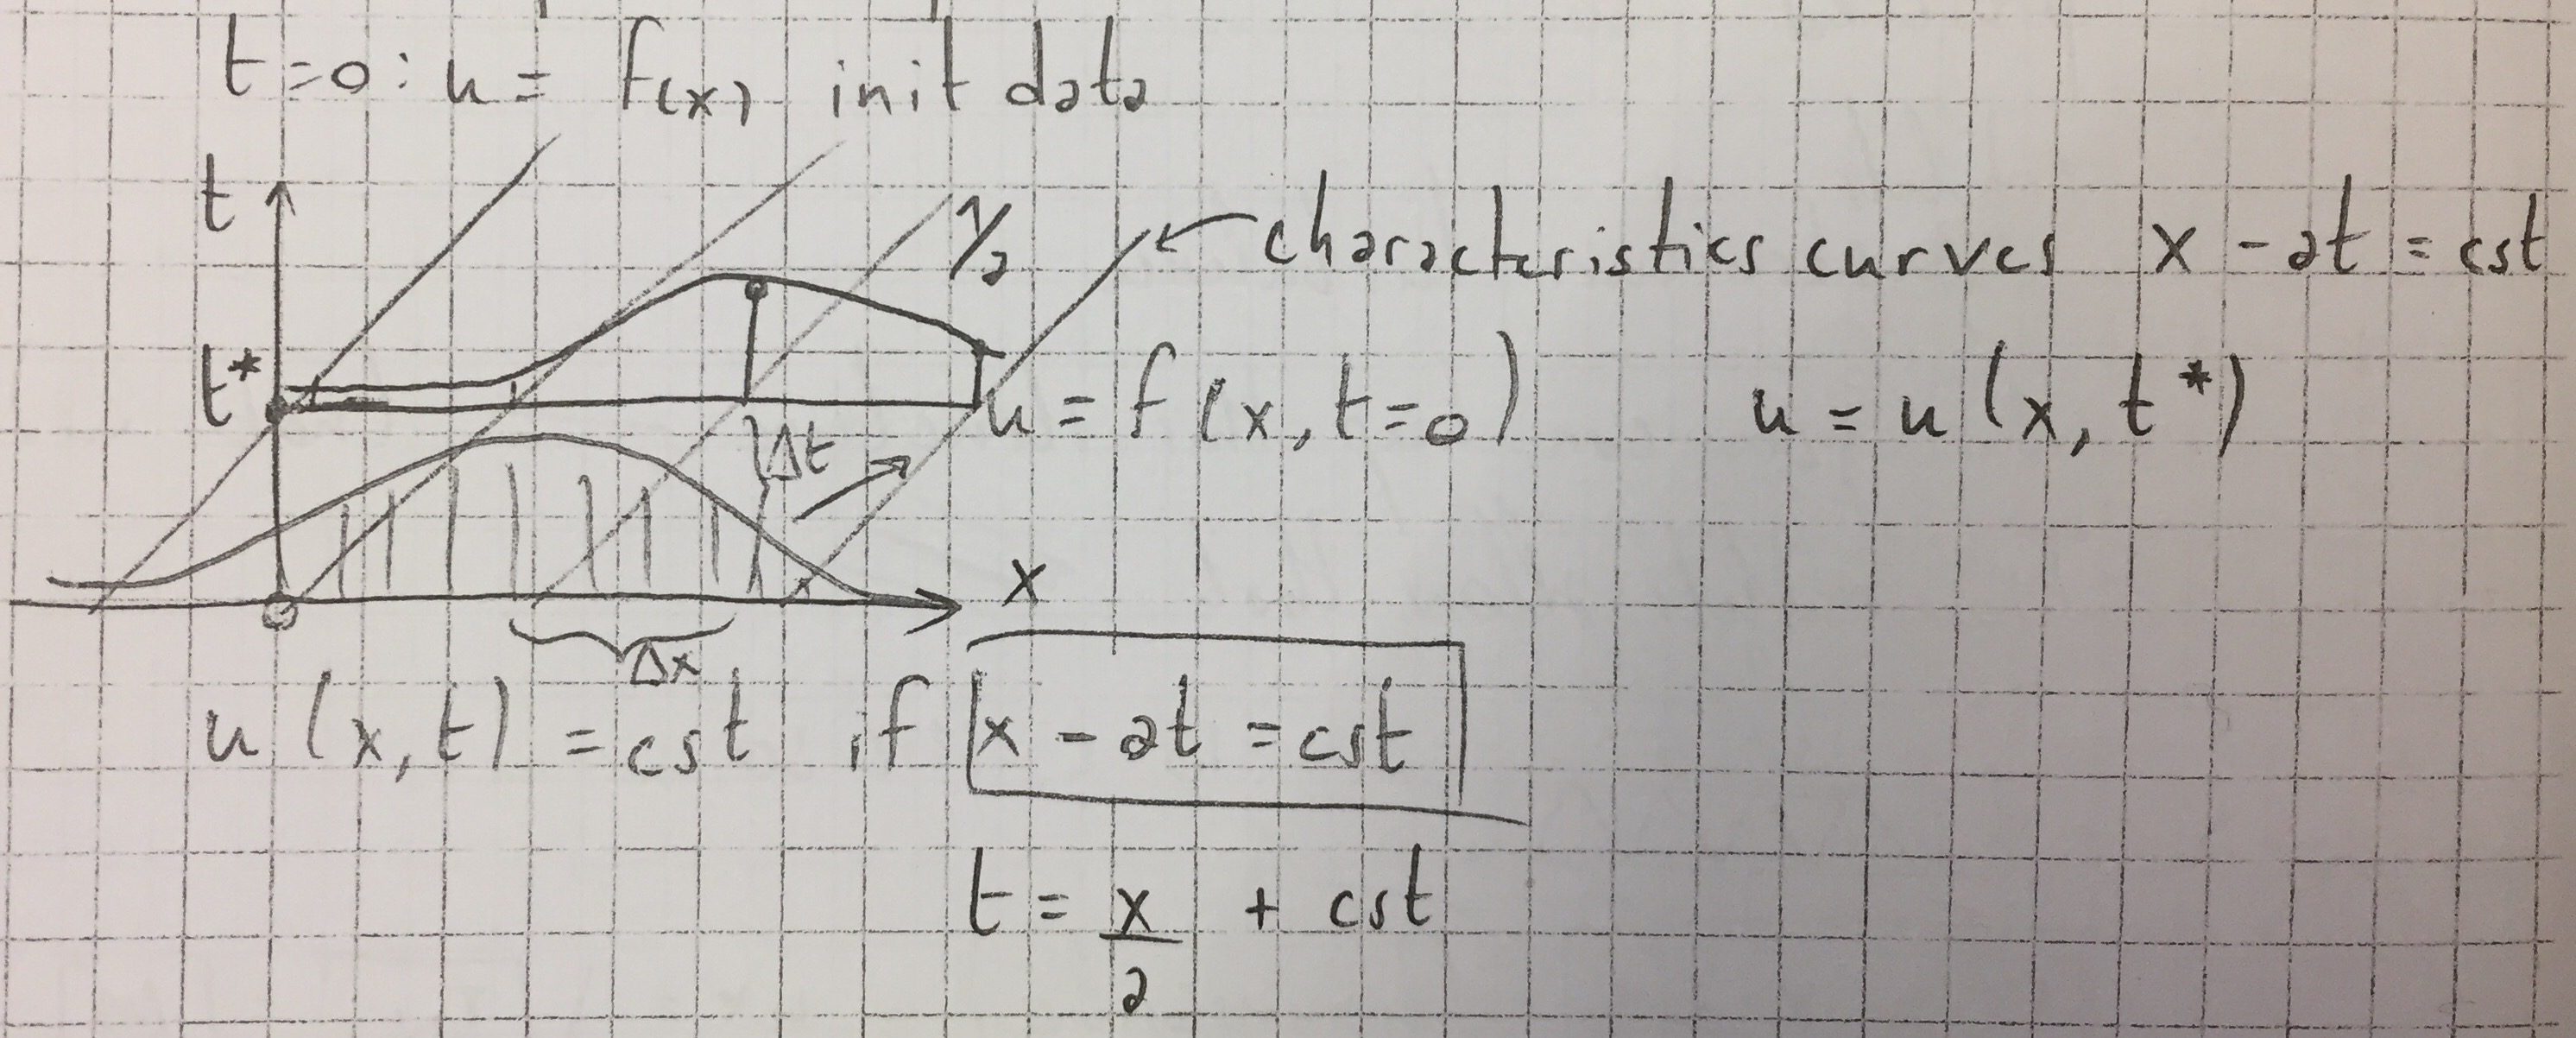
\includegraphics[scale=0.1]{ch8/7}
	\captionof{figure}{}
	\end{center}
	
	Initial wave is shifted on the right. Euler equation in 2D comes from the 1D momentum equation: 
	
	\begin{equation}
	\frac{\D u}{\D t} + u\frac{\D u}{\D x} = \frac{1}{\rho } \mu \frac{\D u^2}{\D  x^2} + \cancel{\frac{1}{\rho }\frac{\D p}{\D x}}
	\end{equation}
	
	Ir the Re number tends to infinity, the right side is canceled and we switch from N-S equations to Euler equation:
	
	\begin{equation}
	\begin{array}{c}
	\frac{\D u}{\D t} + \frac{\D F}{\D x} + \frac{\D G}{\D y} = 0 \\
	u= \left( \begin{array}{c}
	\rho \\
	\rho u\\
	\rho v\\
	\rho E
	\end{array}
	\right)
	\qquad 
	F= \left( \begin{array}{c}
	\rho \\
	\rho u^2 + p\\
	\rho uv\\
	\rho uH
	\end{array}
	\right)
	\qquad 
	u= \left( \begin{array}{c}
	\rho v\\
	\rho uv\\
	\rho v^2 +p\\
	\rho vH
	\end{array}
	\right)
	\end{array}
	\end{equation}
	
	where u is the vector of \textbf{conservative variables}, F and G are the \textbf{flux vectors}, E the total energy and H the total enthalpy. More compact: 
	
	\begin{equation}
	\frac{\D  u}{\D t} + \nabla \bar{\bar{F}} = 0 \qquad \bar{\bar{F}} = (F,G).
	\end{equation}
	
	\wrapfig{10}{l}{5}{0.5}{ch8/1}{ch8/1}
	When stationary, $\nabla \bar{\bar{F}} = 0$. A shock is a discontinuity and derivatives are not defined. They have to satisfy the integral to be a weak solution: 
	
	\begin{equation}
	\int _V \nabla \bar{\bar{F}}\, dV = 0 \Rightarrow \oint _S \bar{\bar{F}}\vec{n} \, dS= 0
	\end{equation}
	
	We can split it into the 4 faces of the surface by considering it infinitely thin (so 2 faces vanish): 
	
	\begin{equation}
	\int _{S_1} \bar{\bar{F}}\vec{n}_1 \, dS + \int _{S_2} \bar{\bar{F}}\vec{n2} \, dS = 0 = [\bar{\bar{F}}\vec{n}]_1^2
	\end{equation}
	
	where the last equality comes from $\vec{n} = \vec{n}_2 = \vec{n}_1$ and the control volume infinitely small. If above condition is satisfied, the discontinuity is a solution of the non-viscous equations: 
	
	\begin{equation}
	\bar{\bar{F}}\vec{n} = F n_x + Gn_y = \left( \begin{array}{c}
	\rho (\vec{u}\vec{n})\\
	\rho u (\vec{u} \vec{n} + pn_x)\\
	\rho v (\vec{u} \vec{n} + pn_y)\\
	\rho H (\vec{u}\vec{n})	
	\end{array}
	\right)
	\end{equation}
	
	The first condition to satisfy, coming from mass conservation, is then: 
	
	\begin{equation}
	\rho _1 u_{n_1} = \rho _2 u_{n_2}
	\end{equation}
	
	The one coming from impulse conservation is: 
	
	\begin{equation}
	[\rho \vec{u}(\vec{u}\vec{n})+p\vec{n}]^2_1 \quad \Rightarrow p_1 + \rho _1 u_{n_1}^2 = p_2 + \rho _2 u_{n_2}^2
	\end{equation}
	
	where we added a scalar product with $\vec{n}$. If we make now the scalar product with the tangential component $\vec{t}$ we find: 
	
	\begin{equation}
	\rho _1 u_{n_1} u_{t_1} = \rho _2 u_{n_2} u_{t_2}\quad \Rightarrow u_{t_1} =u_{t_2}
	\end{equation}
	
	where we used the mass conservation. \textbf{The velocity is conserved along the shock in both sides}.The last equation in the same way gives: 
	
	\begin{equation}
	H_1 = H_2
	\end{equation}
	
	\textbf{conservation of entropy across the shock} like on a streamline. If we consider a discontinuous streamline, $\dot{m} = \vec{u}\vec{n} = 0$ and implies by momentum condition: 
	
	\begin{equation}
	p_1 \vec{u} = p_2 \vec{u} \qquad \Rightarrow p_1 = p_2
	\end{equation}
	
	$un = 0$ is the definition of the \textbf{shear layer}. The density is not conserved with the shock, thus by the perfect gas theory, the temperature too. 
	
\section{Mach waves and characteristics}
	Consider a static source emitting infinitely small perturbations in a standstill fluid. These propagates in all direction with the \textbf{speed of sound}. If the source stands still, the perturbations stay within always larger concentric circles. 
	
	\wrapfig{7}{l}{3}{0.1}{ch8/2}{ch8/2}
	Suppose now that the source moves to the left with $V_\infty < a$. After a certain time $t^*$, the source will move from A to B. But in that interval the first perturbation circle has enlarged from $at^*$ and with center A. If we devide the time interval into 5, we will have a situation like on the figure. We can see that the perturbations are both downstream and upstream of the source.  

	\minifig{ch8/3}{ch8/4}{0.5}{0.4}{0.3}{0.3}
	
	Consider now the case $V_\infty = a$ and the case $V_\infty > a$ represented above. There is now no perturbation upstream the perturbation. In particular, in the first case the perturbation are situated in the half plane downstream the source and the second within a cone of opening $2\mu$ called the \textbf{Mach cone}. From the figure, we can directly deduce: 
	
	\begin{equation}
	\sin \mu = \frac{a}{V_\infty} = \frac{1}{M_\infty}.
	\end{equation}
	
	The area within the cone is the \textbf{area of action} and outside the \textbf{area of silence}. The lines separating both are the \textbf{Mach waves}. 
	
	\wrapfig{7}{l}{6}{0.25}{ch8/5}{ch8/5}
	Now consider the reversed case where the source (an infinitesimal irregularity) is standing still and the fluid is moving. Here also we get the same results. Within the assumption of small perturbations, the following equation (elliptic) is valid for supersonic flows: 
	
	\begin{equation}
	\lambda ^2 \hat{\phi} _{xx} - \hat{\phi}_{yy} = 0 \qquad \lambda ^2 = M_\infty ^2 -1
	\end{equation}
	
	for subsonic, the signs are reversed. The general solution of this equation was: $\hat{\phi} = f(x-\lambda y) + g(x+\lambda y)$. But $\frac{1}{\lambda} = \tan \mu$ and thus: 
	
	\begin{equation}
	\hat{\phi} = f(y - x\tan \mu) + g(y + x \tan \mu)
	\end{equation}
	
	the solution is constant along straight lines of slope $\pm \mu$ which corresponds to the Mach waves. Mach waves are thus characteristics of the \textbf{hyperbolic} equation: 
	
	\begin{equation}
	\hat{\phi} _{xx} = \tan^2 \mu \hat{\phi} _{yy} 
	\end{equation}
	
\subsubsection{Subcritical and supercritical waves}
	\wrapfig{5}{l}{3.5}{0.05}{ch8/8}{ch8/8}
	Consider a wave of height h after one time, the equations are: 
	
	\begin{equation}
	\begin{aligned}
	&\frac{\D }{\D x} (uh) + \frac{\D}{\D y} (vh) = 0\\
	\mbox{x-mom: } &\frac{\D}{\D x } (u^2 + gh) + \frac{\D}{\D y} (uv) = 0\\
	\mbox{y-mom: } &\frac{\D}{\D x } (uv) + \frac{\D}{\D y} (v^2 + gh) = 0
	\end{aligned}
	\end{equation}
	
	where $\sqrt{gh}$ is the speed of waves on water. A relation between Mach and Froude number can be made since $a = \sqrt{\sqrt{\gamma p /\rho}}$: 
	
	\begin{equation}
	M = \sqrt{\frac{u^2 + v^2}{\frac{\gamma p}{\rho}}} \qquad Fr = \sqrt{\frac{u^2 + v^2}{gh}}
	\end{equation}
	
	If $Fr > 1$: supercritical = supersonic, if $Fr < 1$: subcritical = subsonic. 
	
\subsection{Characteristic theory for first order hyperbolic system of partial differential equations (PDE)}

\subsubsection{a cst}	
	The prototype equation is the linear scalar wave equation: 
	
	\begin{equation}
	\frac{\D u}{\D x} + a \frac{\D u}{\D y} = 0
	\end{equation}
	
	\wrapfig{9}{l}{6}{0.2}{ch8/9}{ch8/9}
	where x is the "time-like" coordinate, y the "space-like" one, a is the convection speed and the initial condition is $u(x,0) = f(y)$. The solution of this is a wave: 
	\begin{equation}
	u(x,y) = f(y-ax) = f(q(x,y))
	\end{equation}
	If $y-ax = cst$ then $u= cst$, which corresponds to $\frac{dy}{dx}$ \textbf{characteristic curves}. Consider on the figure that left is inlet and right is outlet, then the wave moves to right with speed $\frac{\Delta y}{\Delta x} = a$. 
	
\subsubsection{a linear}
	If a is not a constant but respects $a = a(x,y)$ the results are similar. 
	
	\begin{proof}
	Since the coordinate y is expressed like $y = ax + cst$, $u$ only depends on x. So if $\frac{du}{dx} = 0$ this means that $u = cst$. Let's compute: 
	
	\begin{equation}
	\frac{du(y(x),x)}{dx} = \frac{\D u}{\D y} \frac{d y}{dx} + \frac{\D u}{\D x} = \frac{\D u}{\D x} -a \frac{\D u}{\D y} = 0
	\end{equation}
	
	which is satisfied since we retrieve the wave equation and u is a solution. 
	\end{proof}
	
	\wrapfig{7}{l}{5}{0.2}{ch8/10}{ch8/10}
	The result is shown here, the only change is that the wave is deformed since the propagation speed is not constant. 
	
	\subsubsection{a non linear}
	In the case a is expressed as $a(u,x,y)$ nothing changes, $\frac{dy}{dx} = a(u,x,y)$ are the characteristics and $u = cst$ along them. The proof is same as before, $y = y(x)$ on the characteristics and $\frac{du}{dx} = 0$. The only change is a depending on 3 variables.  
	
	\exemple{
	
	Consider
	\begin{equation}
	a = u \qquad \frac{\D u}{\D x} + u \frac{\D u }{\D y} = 0 
	\end{equation}
		
	The solution $u=cst$ on characteristic curves $\frac{dy}{dx} = u$. This means that characteristics are straight lines since $u=cst$ along them and is the slope. They only differs from the initial data $u = f(y)$ at $x = 0$. There are 2 cases to consider since the wave can be converging or diverging as shown on below figures. 
	
	\minifig{ch8/11}{ch8/12}{0.3}{0.3}{0.3}{0.3}
	
	The first one corresponds to an expansion wave, the characteristics are diverging. The wave is smoothened during its expansion on x-axis. In the second case, the characteristics are converging and we call it compression wave. This leads to wave steepening. At the characteristics intersection we have an \textbf{overturning wave} as shown, this is a tripled value solution. 
	
	\begin{center}
	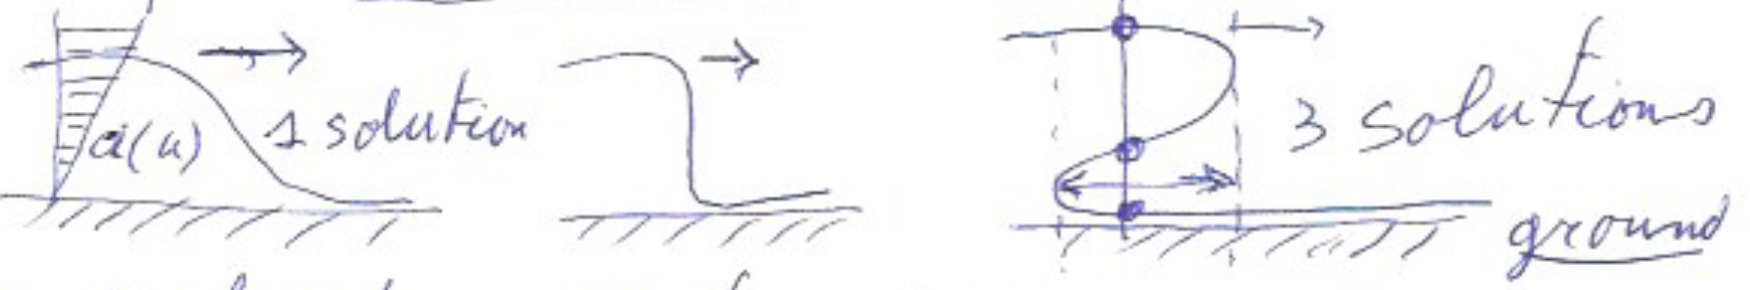
\includegraphics[scale=0.3]{ch8/13}
	\captionof{figure}{}
	\end{center}		
	
	This is due to the fact that the wave moves slower near the ground (ex: wave at the beach). But with Euler equations this is not permitted since the solution has to be unique and thus can be interpreted as a shock wave. 
	}
	
\subsubsection{Linear system of 2 first order PDE}
	This case corresponds to equations as: 
	
	\begin{equation}
	\frac{\D U}{\D x} + A \frac{\D U}{\D y} = 0 \qquad U = \left(\begin{array}{c}
	u\\
	v
	\end{array}
	\right)
\end{equation}			
	and A is a $4\times 4$ matrix. 
	
	\exemple{
	
	Consider the \textbf{second order D'Alembert wave equation}: 
	
	\begin{equation}
	\phi _{xx}-c^2 \phi _{yy} = 0
	\label{eq:dalembert}
\end{equation}		
	
	The solution of this equation is: 
	
	\begin{equation}
	\phi (x,y) = F_1(x-cx ) +  F_1(x + cx )
	\end{equation}
	where $F_1$ is the forward moving wave with speed +c and the backward for the other. There are 2 initial data to give, $F_1(y)$ and $F_2(y)$: $\phi (y,0) = F_1(y) + F_2(x)$. Let's solve \autoref{eq:dalembert} in a different way by defining: 
	
	\begin{equation}
	u = \phi _x, v = \phi _y \qquad \Rightarrow \begin{aligned}
	&u_x - c^2 v_y = 0 \\
	&v_x - u_y = 0
	\end{aligned}
	\end{equation}
	
	and in the matrix form: 
	
	\begin{equation}
	\frac{\D}{\D x} \left( 
	\begin{array}{c}
	u\\
	v	
	\end{array}
	\right)
	= 
	\left( 
	\begin{array}{cc}
	0 & -c^2\\
	-1 & 0	
	\end{array}
	\right)
	\frac{\D }{\D y}
	\left( 
	\begin{array}{c}
	u\\
	v	
	\end{array}
	\right)
	= 0
	\end{equation}
	
	\textbf{The eigenvalues of A are the wave speeds} $\bm{\pm c}$. Thus define the characteristic curves, here 2 families of curves. 
	
	\begin{center}
	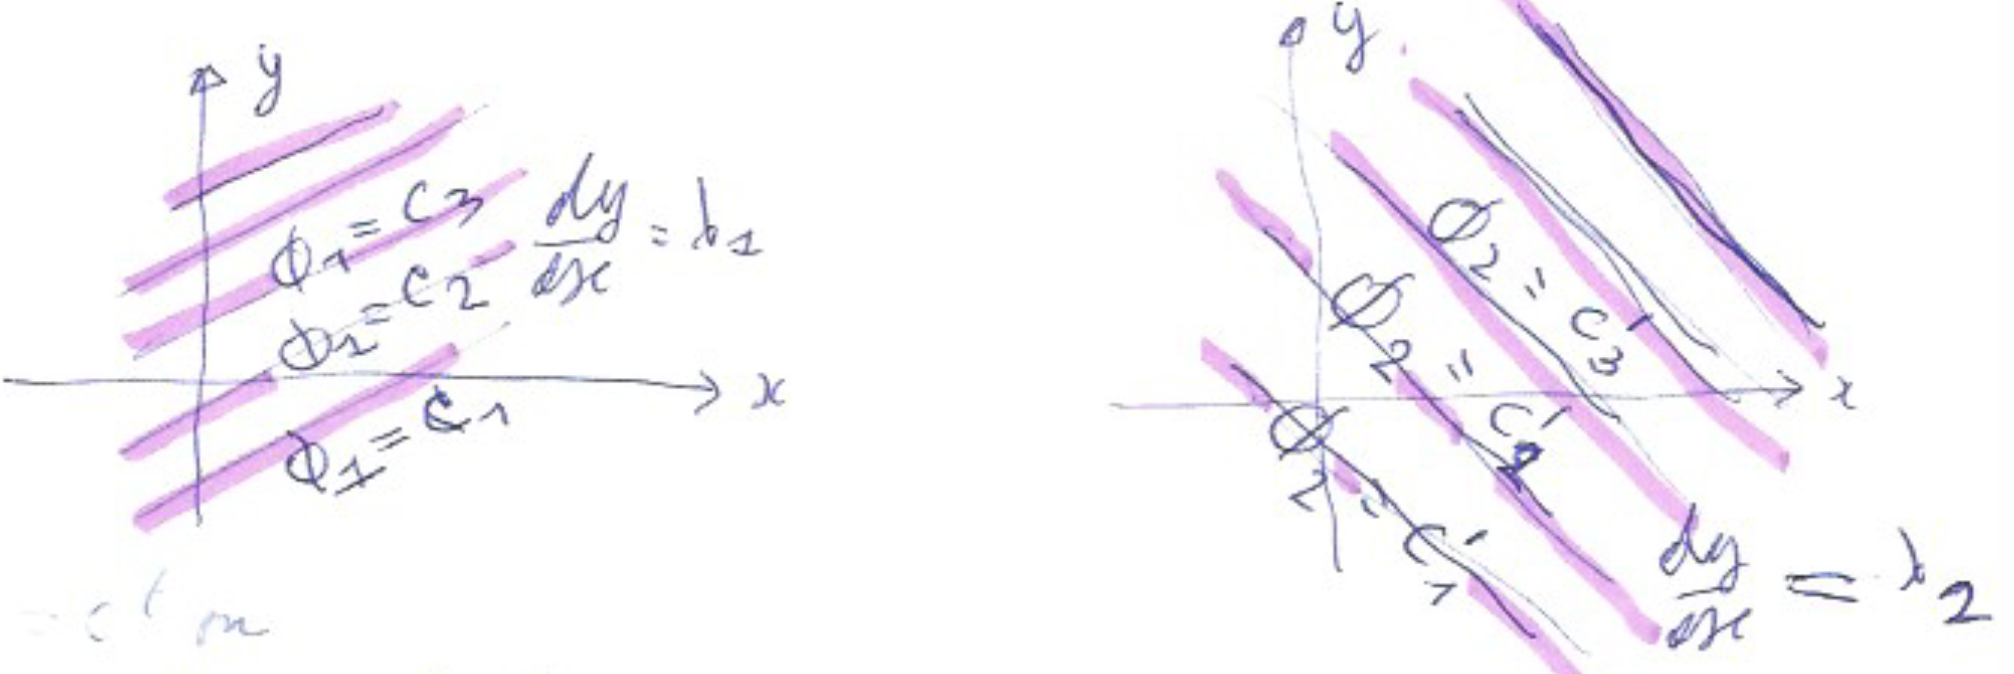
\includegraphics[scale=0.3]{ch8/14}
	\captionof{figure}{}
	\end{center}	 
	
	Hence the solution is: 
	
	\begin{equation}
	\phi (x,y) = \phi _1 (x,y) + \phi _2 (x,y) = F_1 (y-cx) + F_2 (y+cx)
	\end{equation}
	
	with $\phi _{1,2} (x,y) = F_{1,2} = cst$ on respectively family 1 and 2. Be careful that this only works if $\lambda_j (A) \in \mathcal{R}$, definition of hyperbolic system of PDE.
	}
	
	\exemple{
	Consider now the elliptic equation: 
	
	\begin{equation}
	\phi _{xx} + c^2 \phi _{yy} = 0
	\end{equation}
	
	For the same procedure as above, we obtain complex eigenvalues: $\lambda = \pm ic$. So if $\lambda _j (A)$ are complex with non zero imaginary part, the system is called \textbf{elliptic}.
	}
	
	\ \\ Note that for a 3rd order system (hybrid system), the eigenvalues can be 1 real + 2 complex conjugate or 3 real (hyperbolic). Elliptic is impossible. If 4th order, elliptic, thus \textbf{biharmonic}. 
	
	\exemple{
	Linearized potential flow: 
	
	\begin{equation}
	\phi _{yy} - \frac{1}{M^2_\infty - 1} \phi _{xx} = 0 
\end{equation}		

	For supersonic flows, we have hyperbolic wave equation and for subsonic we have an elliptic diffusion equation since we have $c^2 = \pm \frac{1}{M^2_\infty - 1} \Rightarrow \lambda _1^\pm = \pm c$ and $\lambda_2^\pm = \pm ic$. Below is represented the supersonic case. 
	
	\begin{center}
	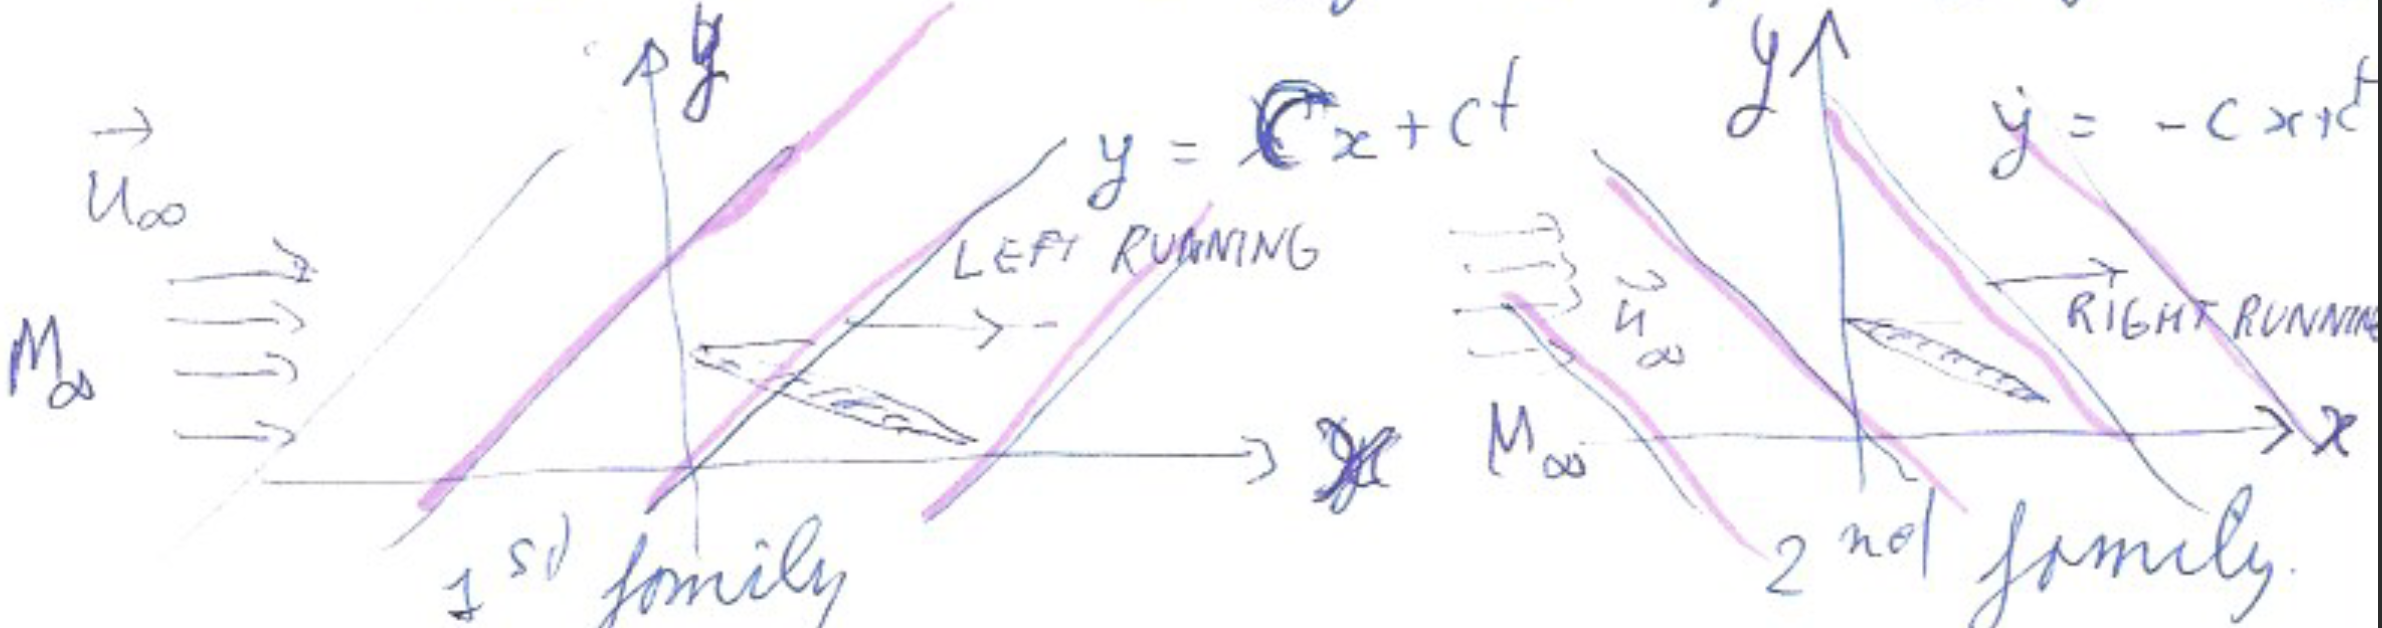
\includegraphics[scale=0.3]{ch8/15}
	\end{center}
	
	Depending on the initial conditions we are in 1 or 2, if $F_1(x) = 0$ first and same for the inverse. In this case the characteristic curves are called the \textbf{Mach lines} and $\tan \mu = \frac{1}{\sqrt{M^2_\infty - 1}}$
	}
	
\subsubsection{Method of characteristics for a 1st order system of PDE for constant coefficients}
	We intend to solve the hyperbolic equation: 
	
	\begin{equation}
	\frac{\D U}{\D x} + A \frac{\D U}{\D y} = 0
	\end{equation}
	
	The idea is to convert this to a decoupled system of 2 scalar wave equations by diagonalizing: 
	
	\begin{equation}
	LAR = D = \left( 
	\begin{array}{cc}
	\lambda _1 & 0\\
	0 & \lambda _2
	\end{array}
	\right) \qquad R = (r_1 \ r_2) \qquad L = (l_1 \ l_2) ^t
	\end{equation}
	
	where $r_i$ are column eigenvectors and $l_i$ row eigenvectors with $L = R^{-1}$. For this, we multiply the system of equation by L and we add RL since LR = I: 
	
	\begin{equation}
	L\frac{\D U}{\D x} + LARL \frac{\D U}{\D y} = 0 \quad \Rightarrow 	\frac{\D LU}{\D x} + LAR \frac{\D LU}{\D y} = 0
	\end{equation}
	
	and we define the \textbf{characteristic variables}: $W = LU = (w_1 \ w_2)^t$ ad we get the decoupled system: 
	
	\begin{equation}
	\frac{\D W}{\D x} + D \frac{\D W}{\D y} = 0
	\end{equation}
	
	The solution of the first and second are: 
	
	\begin{equation}
	\begin{aligned}
	w_1(x,y) = w(y- \lambda _1 x) \quad w_1(x,y) = cst \ on \ \frac{\d y}{dx} = \lambda _1\\
	w_2(x,y) = w(y+ \lambda _2 x) \quad w_2(x,y) = cst \ on \ \frac{\d y}{dx} = \lambda _2
	\end{aligned}
	\end{equation}
	
	\wrapfig{6}{l}{5}{0.3}{ch8/16}{ch8/16}
	The constant is fixed by the initial data on $x=0$: 
	\begin{equation}
	w_1(x_P, y_P) = w_1^* (x_A, y_A)\\
	w_2(x_P, y_P) = w_2^* (x_B, y_B)
	\end{equation}
	
	So to find the solution in P: 
	
	\begin{enumerate}
	\item Find the two characteristic curves
	\item Trace back to the initial data to find the constants
	\item Transform back to the variable U: 
	
	\begin{equation}
	U_P = RW_P
	\end{equation}
	\end{enumerate}
	
\subsubsection{Application to the potential flow}
	The characteristic curves are: 
	
	\begin{equation}
	C^\pm: \quad \left(\frac{dy}{dx}\right)^\pm = \pm \frac{1}{\sqrt{M^2_\infty -1}} = \tan (\pm \mu _\infty) 
	\end{equation}
	
	There are two ways of computing the eigenvectors: solving $AR = RD$  or $Ar_j = \lambda _jr_j $and $LA = DL$ or $l_jA = \lambda _jl_j $for $r_j$ and $l_j$ respectively, we prefer the second. In our case: 
	
	\begin{equation}
	l_1 A = \lambda _1 l_1 \qquad \Rightarrow (\alpha \ \beta) \left(
	\begin{array}{cc}
	0 & -c^2\\
	-1 & 0
	\end{array}
	\right)
	= +c (\alpha \beta)
	\end{equation}
	
	After solving we find: $l_1 = c^t(1 \ -c)$ and $l_2 = c^t(1 \ +c)$. The characteristic variable $W = LU$ is: 
	
	\begin{equation}
	\begin{aligned}
	w_1 = l_1 U = c^t (u  -\frac{1}{\sqrt{M_\infty^2 -1}} v)\\
	w_2 = l_2 U = c^t (u  +\frac{1}{\sqrt{M_\infty^2 -1}} v)
	\end{aligned}
	\end{equation}
	
	and these functions are constant along the characteristic curves and are called \textbf{Riemann invariant}. 
	
	\wrapfig{8}{l}{5}{0.3}{ch8/17}{ch8/17}
	Remember that u and v are the perturbation velocities. To compute them on the lower side of the profile we use $C^-$: 
	
	\begin{equation}
	u_P + \frac{v_P}{\sqrt{M^2_\infty -1}} = u_\infty + \frac{v_\infty}{\sqrt{M^2_\infty -1}} = 0 
	\end{equation}
	
	the second member is null since there is no perturbation at $\infty$. There are still the boundary conditions: 
	
	\begin{equation}
	\frac{v_P}{V_\infty + u_P}= \tan \theta _{wall} \qquad \Rightarrow \frac{v_P}{V_\infty} \approx \theta _{wall}
	\end{equation}
	
	So that we can find the velocities:
	
	\begin{equation}
	v^-_P = V_\infty \theta^- _{wall} \quad \Rightarrow u_P^- = \frac{V_\infty\theta ^-_{wall}}{\sqrt{M_\infty ^2 - 1}} \quad \Rightarrow c_P^- = \frac{-2 \theta ^-_{wall}}{\sqrt{M_\infty ^2 - 1}}
	\end{equation}
	
	Which is the previously seen \textbf{Ackaret's law}. Same process applied to the upper side gives the same results with inverted signs. \\
	
	For non-linear PDE's, the idea is exactly the same, the only difference is that the variable U will appear in the $\lambda$, the $L(U)$ and that the decoupled equations have the form: 
	
	\begin{equation}
	\frac{\D w_1}{\D x} + \lambda _1(U) \frac{\D w_1}{\D y} = 0 
	\end{equation}
	
	This is an ODE along the characteristic curve: $\frac{dw_1}{ds} = 0$ with $ds = \frac{\D}{\D x} + \lambda_1(U) \frac{\D}{\D y}$.
	
\subsection{Characteristic theory for 2D supersonic potential flow}
	Consider the following system of potential flow equations: 
	
	\begin{equation}
	\left\{
	\begin{aligned}
	&\left( 1 - \frac{u^2}{a^2} \right) u_x - \frac{uv}{a^2} (u_y + v_x) + \left( 1  \frac{v^2}{a^2} \right) v_y = 0\\
	& v_x - u_y = 0
	\end{aligned}
	\right.
	\end{equation}
	
	This can be put in matrix form as follows: 
	
	\begin{equation}
	\frac{\D}{\D x} 
	\left( 
	\begin{array}{c}
	u\\
	v
	\end{array}
	\right)
	+ 
		\left( 
	\begin{array}{ccc}
	\frac{-2uv/a^2}{1-u^2/a^2} & \frac{1-v^2/a^2}{1-u^2/a^2}\\
	-1 & 0
	\end{array}
	\right)
		\frac{\D}{\D y} 
	\left( 
	\begin{array}{c}
	u\\
	v
	\end{array}
	\right)
	\end{equation}
	
	Now we do like in previous section, compute the eigenvalues:
	
	\begin{equation}
	\begin{aligned}
	&\lambda ^2 \left( 1-\frac{u^2}{a^2} \right) + \frac{2 uv}{a^2}\lambda + \left(1-\frac{v^2}{a^2} \right) = 0\\
	&\Delta = - 1 + \frac{u^2 + v^2}{a^2} \quad \Rightarrow \lambda ^\pm = \frac{-uv\pm a^2 \sqrt{M^2 - 1}}{a^2 - u^2} \in \mathcal{R}
	\end{aligned}
\end{equation}	 

	where $\lambda^\pm \in \mathcal{R}$ since $M>1$. We can find after computations that: 
	
	\begin{equation}
	\lambda ^\pm = \tan (\theta \pm \mu )
	\end{equation}
	
	where $\theta$  is the flow angle and $\mu $ the Mach angle with: $\sin \mu = \frac{1}{M}, \tan \theta = \frac{u}{v}$  and $\tan \mu = \frac{1}{\sqrt{M^2-1}}$.  The curves are thus: 
	
	\begin{equation}
	C^+: \left(\frac{dy}{dx}\right)^+ = \tan (theta + \mu) \qquad C^-: \left(\frac{dy}{dx}\right) ^- = \tan (theta - \mu )
	\end{equation}
	
	\begin{center}
	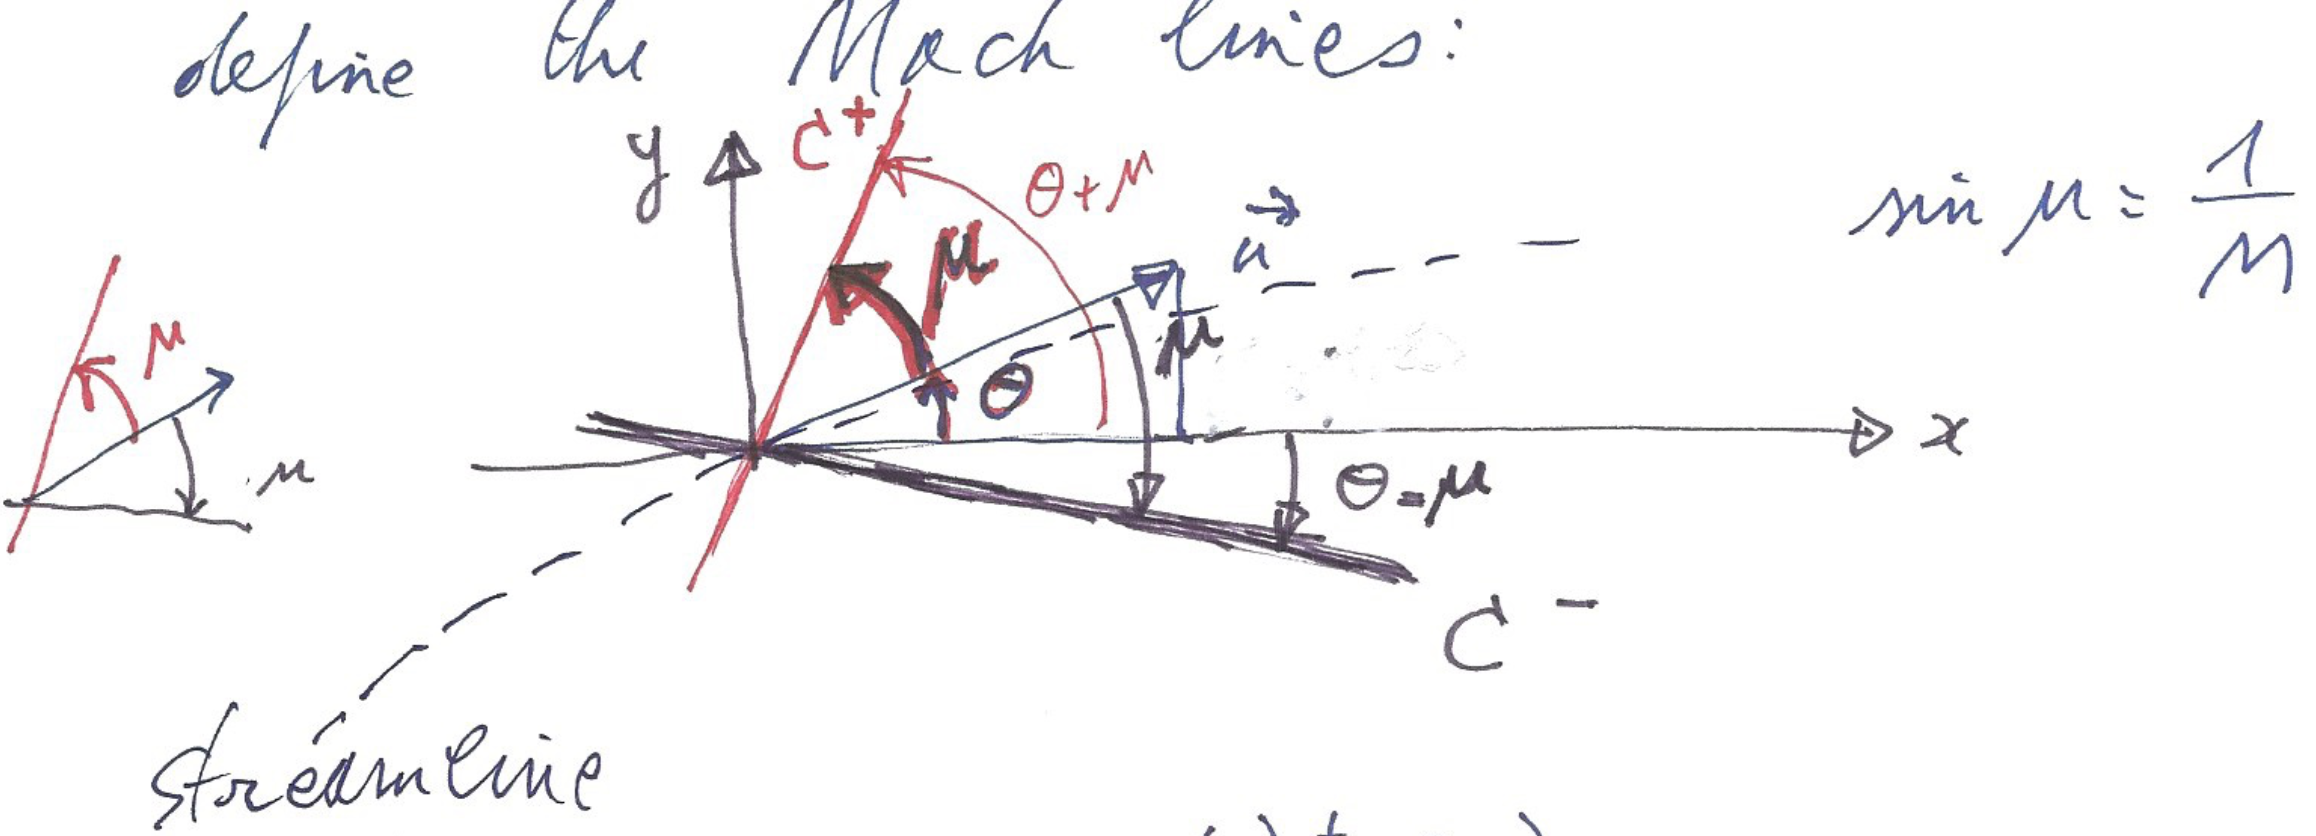
\includegraphics[scale=0.2]{ch8/18}
	\end{center}
	
	Now as the eigenvalues are real, we can diagonalize by finding the left eigenvectors and computing $W = LU$, where $L = (l^+ \ l^-)^t$ such that for "+": 
	
	\begin{equation}
	\frac{\D W^+}{\D x} + D\frac{\D W^+}{\D y} = 0
	\end{equation}
	
	We get a decoupled system of equation. To find L, the same method as previously is used, \textbf{a trick is to choose} $\bm{\sigma = a^2 - u^2}$ \textbf{and to compute} \bm{$\mu$} \textbf{using the system of equation} $\bm{LA = DL}$. We get: 
	
	\begin{equation}
	l^+ = (a^2 - u^2\quad -uv +\sqrt{M^2 -1})
	\end{equation}
	
	The equation can be rewritten as a derivative along the streamline: 
	
	\begin{equation}
	\frac{d W^+}{d s^+} =  0 \qquad \Rightarrow l^+ \frac{d U}{d s^+} = 0 = (a^2 - u^2 )\frac{d u}{d s^+} + (-uv + a^2\sqrt{M^2-1})\frac{dv}{ds^+}
	\end{equation}
	
	Now we can use a transformation $(u,v) \rightarrow (M, \theta)$: 
	
	\begin{equation}
	u = a M\cos \theta \qquad v = a M \sin \theta \qquad a_t = a^2 \left( 1+\frac{\gamma - 1}{2} M^2 \right)
	\end{equation}
	
	where the last equation comes from the total enthalpy, $a = \sqrt{\gamma R T} = \sqrt{\frac{\gamma p}{\rho}}$ and $\frac{c_p}{c_p - c_v}= \frac{\gamma}{\gamma - 1}$: 
	
	\begin{equation}
	\begin{array}{c}
	H = cst = h + \frac{u^2 + v^2}{2} \qquad \Leftrightarrow \frac{\gamma}{\gamma R}c_p T + \frac{u^2+v^2}{2} = c_p T_T \frac{\gamma R}{\gamma R} \\
	\Leftrightarrow \frac{a^2 c_p}{\gamma R} + \frac{u^2 + v^2}{2} = \frac{a^2_t c_p}{\gamma R} \qquad \Leftrightarrow a^2 \left( 1 + M\frac{\gamma -1 }{2} \right) = a^2_t
	\end{array}
	\end{equation}
	
	Then when we solve for $M, \theta$, we get: 
	
	\begin{equation}
	\frac{\sqrt{M^2-1}}{M \left(1+\frac{\gamma -1}{2}M^2\right)}\frac{dM}{ds^+} - \frac{d\theta }{ds^+} = 0
	\end{equation}
	
	And if we integrate this and define the \textbf{Prandtl-Meyer function} \bm{$\nu (M)$}, we have for the Riemann invariants: 
	
	\begin{center}
	\theor{
	\begin{equation}
	C^+: - \nu (M) = \theta = cst = K^+ (M,\theta) \qquad C^-:  \nu (M) = \theta = cst = K^- (M,\theta) 
	\end{equation}
	}
	\end{center}
	
	\minifig{ch8/19}{ch8/20}{0.2}{0.2}{0.49}{0.49}	
	
	The situation is represented above, remark that the points P and Q depends on all the points upstream them outside the cone. Since the characteristics slope depends on the local $M$ and $\theta$,  for the \textbf{method of characteristics} one has to compute all the solutions on $C^\pm$ upstream P to compute the solution in P. 
	
\subsection{Simple waves or simple wave solutions}
	A simple wave solution is a solution for which the Riemann invariant is constant on the whole space (x,y)	and not only on the characteristics. There exiss two types since we have 2 families of characteristics. 
	
	\begin{center}
	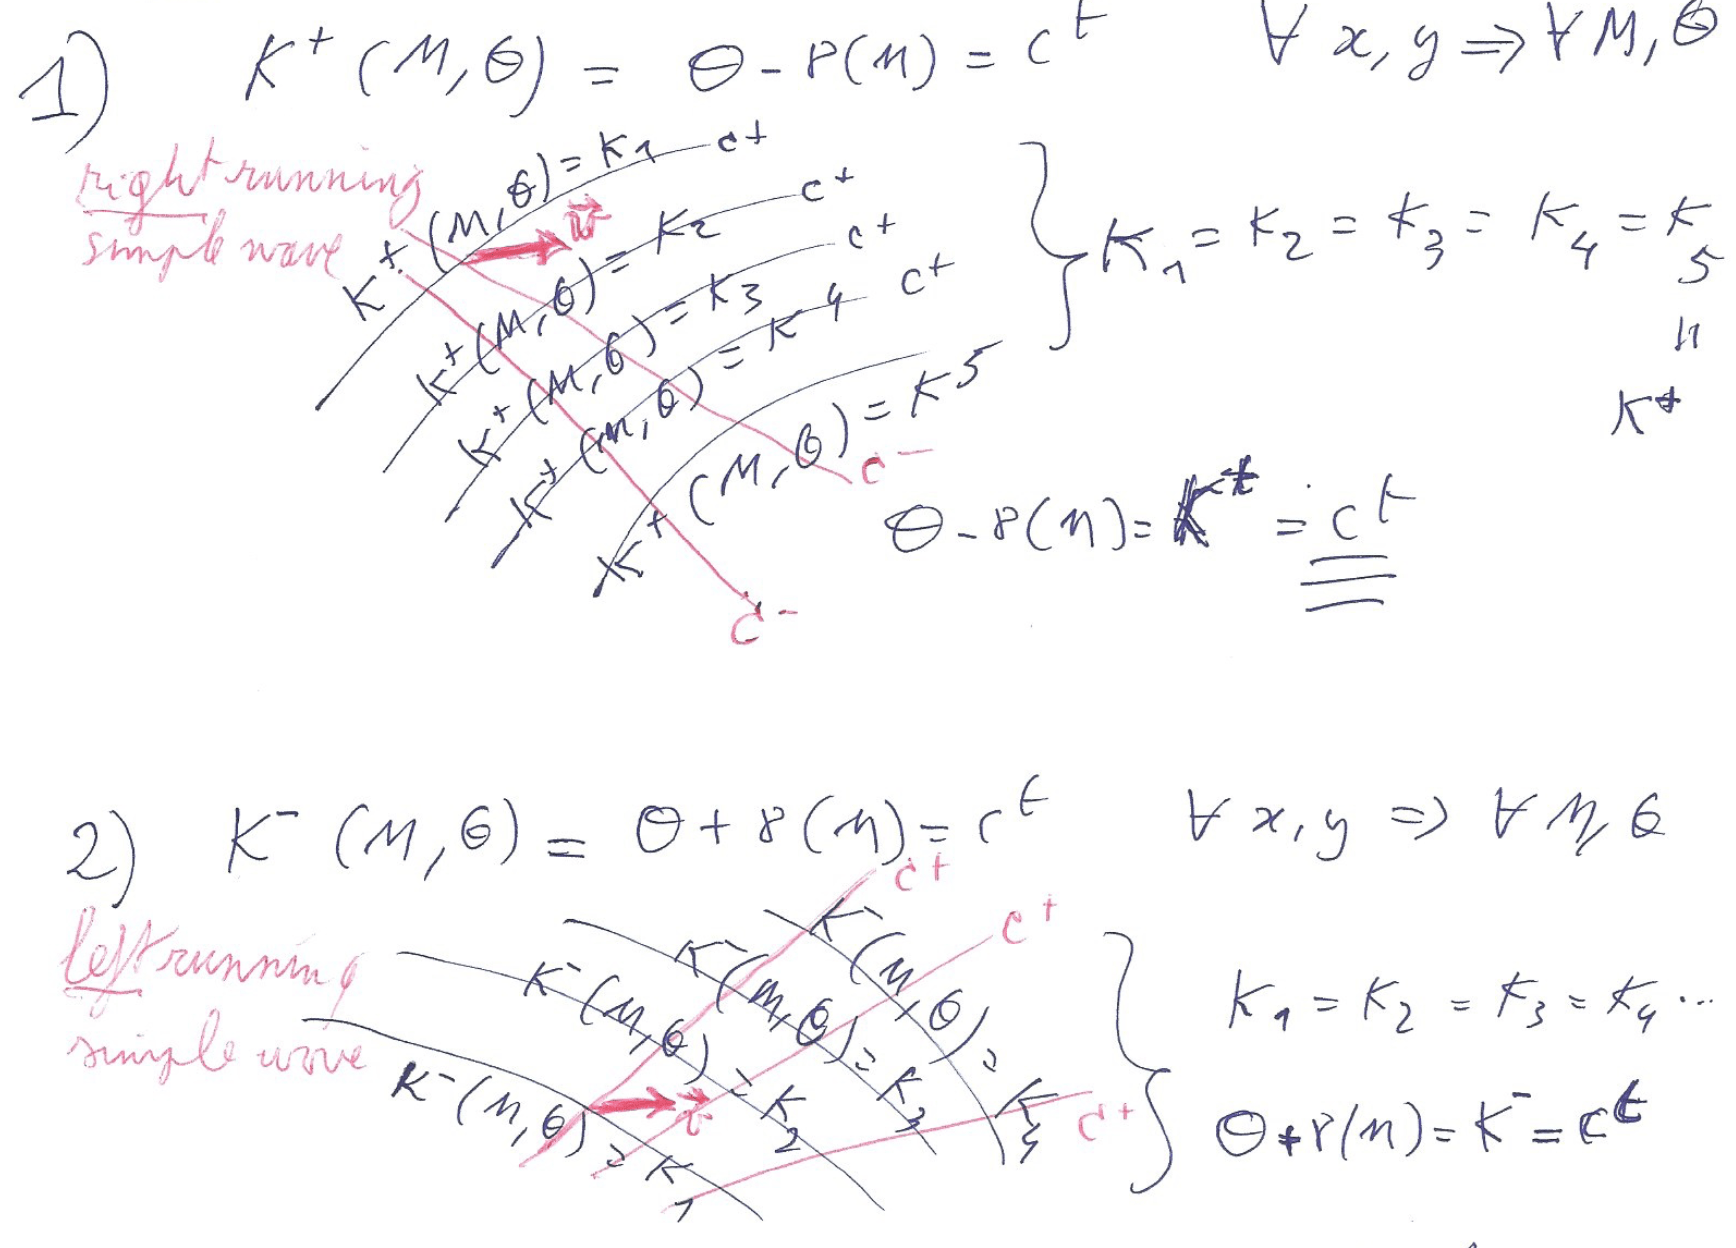
\includegraphics[scale=0.15]{ch8/21}
	\captionof{figure}{}
	\end{center}
	
	It is easy to see that the slope of $C^-$ and $C^+$ in respectively case 1 and 2 is constant, for example for case 2: 
	
	\begin{equation}
	C^+ : \theta - \nu (M) = {Cst}_1 \qquad \mbox{but } \theta + \nu(M) {Cst}_2\qquad \Rightarrow (\theta  , nu)= cst
	\end{equation}
	
\subsubsection{Example}
	\wrapfig{9}{l}{7.75}{0.12}{ch8/22}{ch8/22}	
	Consider the simple wave equation: $\nu (M) +\theta = Cst$ $\forall x,y$ for a supersonic expansion around a bend. This is a type 2 since the initial condition at $\infty$ are defined for $C^-$. 
	
	\paragraph{Computation on the wall P}
	We know that $\theta _\infty = 0$ and that $\theta _P = \theta _{wall,p}$ such that on $C^-$ we have: 
	\ \\
	
	\begin{equation}
	\nu (M_P) + \theta _P = \nu (M_\infty) + \theta _\infty \qquad \Rightarrow \nu (M_P) = \nu (M_\infty) - \theta _{wall,p}
	\end{equation}
	
	and the Mach number on P can be found by inverting: $M_P = \nu ^(\nu (M_\infty) - \theta _{wall,p})$.
	
	\paragraph{Once \bm{$M_P, \theta _P$} are known} We compute the slope of $C^+$: 
	
	\begin{equation}
	\left(\frac{dy}{dx} \right)^+ = \tan (\theta _P + \mu _P ) \qquad \mu _P = \arcsin \left( \frac{1}{M}\right)
	\end{equation}
	
	On this curve, $\theta$ and $M$ are constant and equal to the ones on P.
	
	\paragraph{The \bm{$C^+$} curve forms a diverging fan} Indeed along the wall we have $\theta _w \searrow, \nu (M_w) \nearrow \Rightarrow M _w \nearrow$.
	
	\subsubsection{Limit case}
	\wrapfig{17}{l}{6}{0.15}{ch8/23}{ch8/23}
	There exist a limit downstream velocity: 
	
	\begin{equation}
	h = c_pT_t = c_p T + \frac{u^2 + v^2}{2} = cst
	\end{equation}
	
	We can see that a max velocity can be obtained if $T = 0$: $V_{lim}^2 = c_p T_t$ and the corresponding Mach number is $M_{lim} = \frac{V_{lim}}{\sqrt{\gamma RT}} = \infty$ ($a_{lim}=0$). In that case the Mach angle is 
	
	\begin{equation}
	\mu = \arcsin \left( \frac{1}{\infty} \right) = 0
	\end{equation}
	
	This means that the \textbf{Mach line collapse with the streamline}. In fact, we will have an inviscid separation downstream and there will be a \textbf{vacuum} where no molecule can be. This is shown on \autoref{ch8/24}.
	
	\begin{center}
	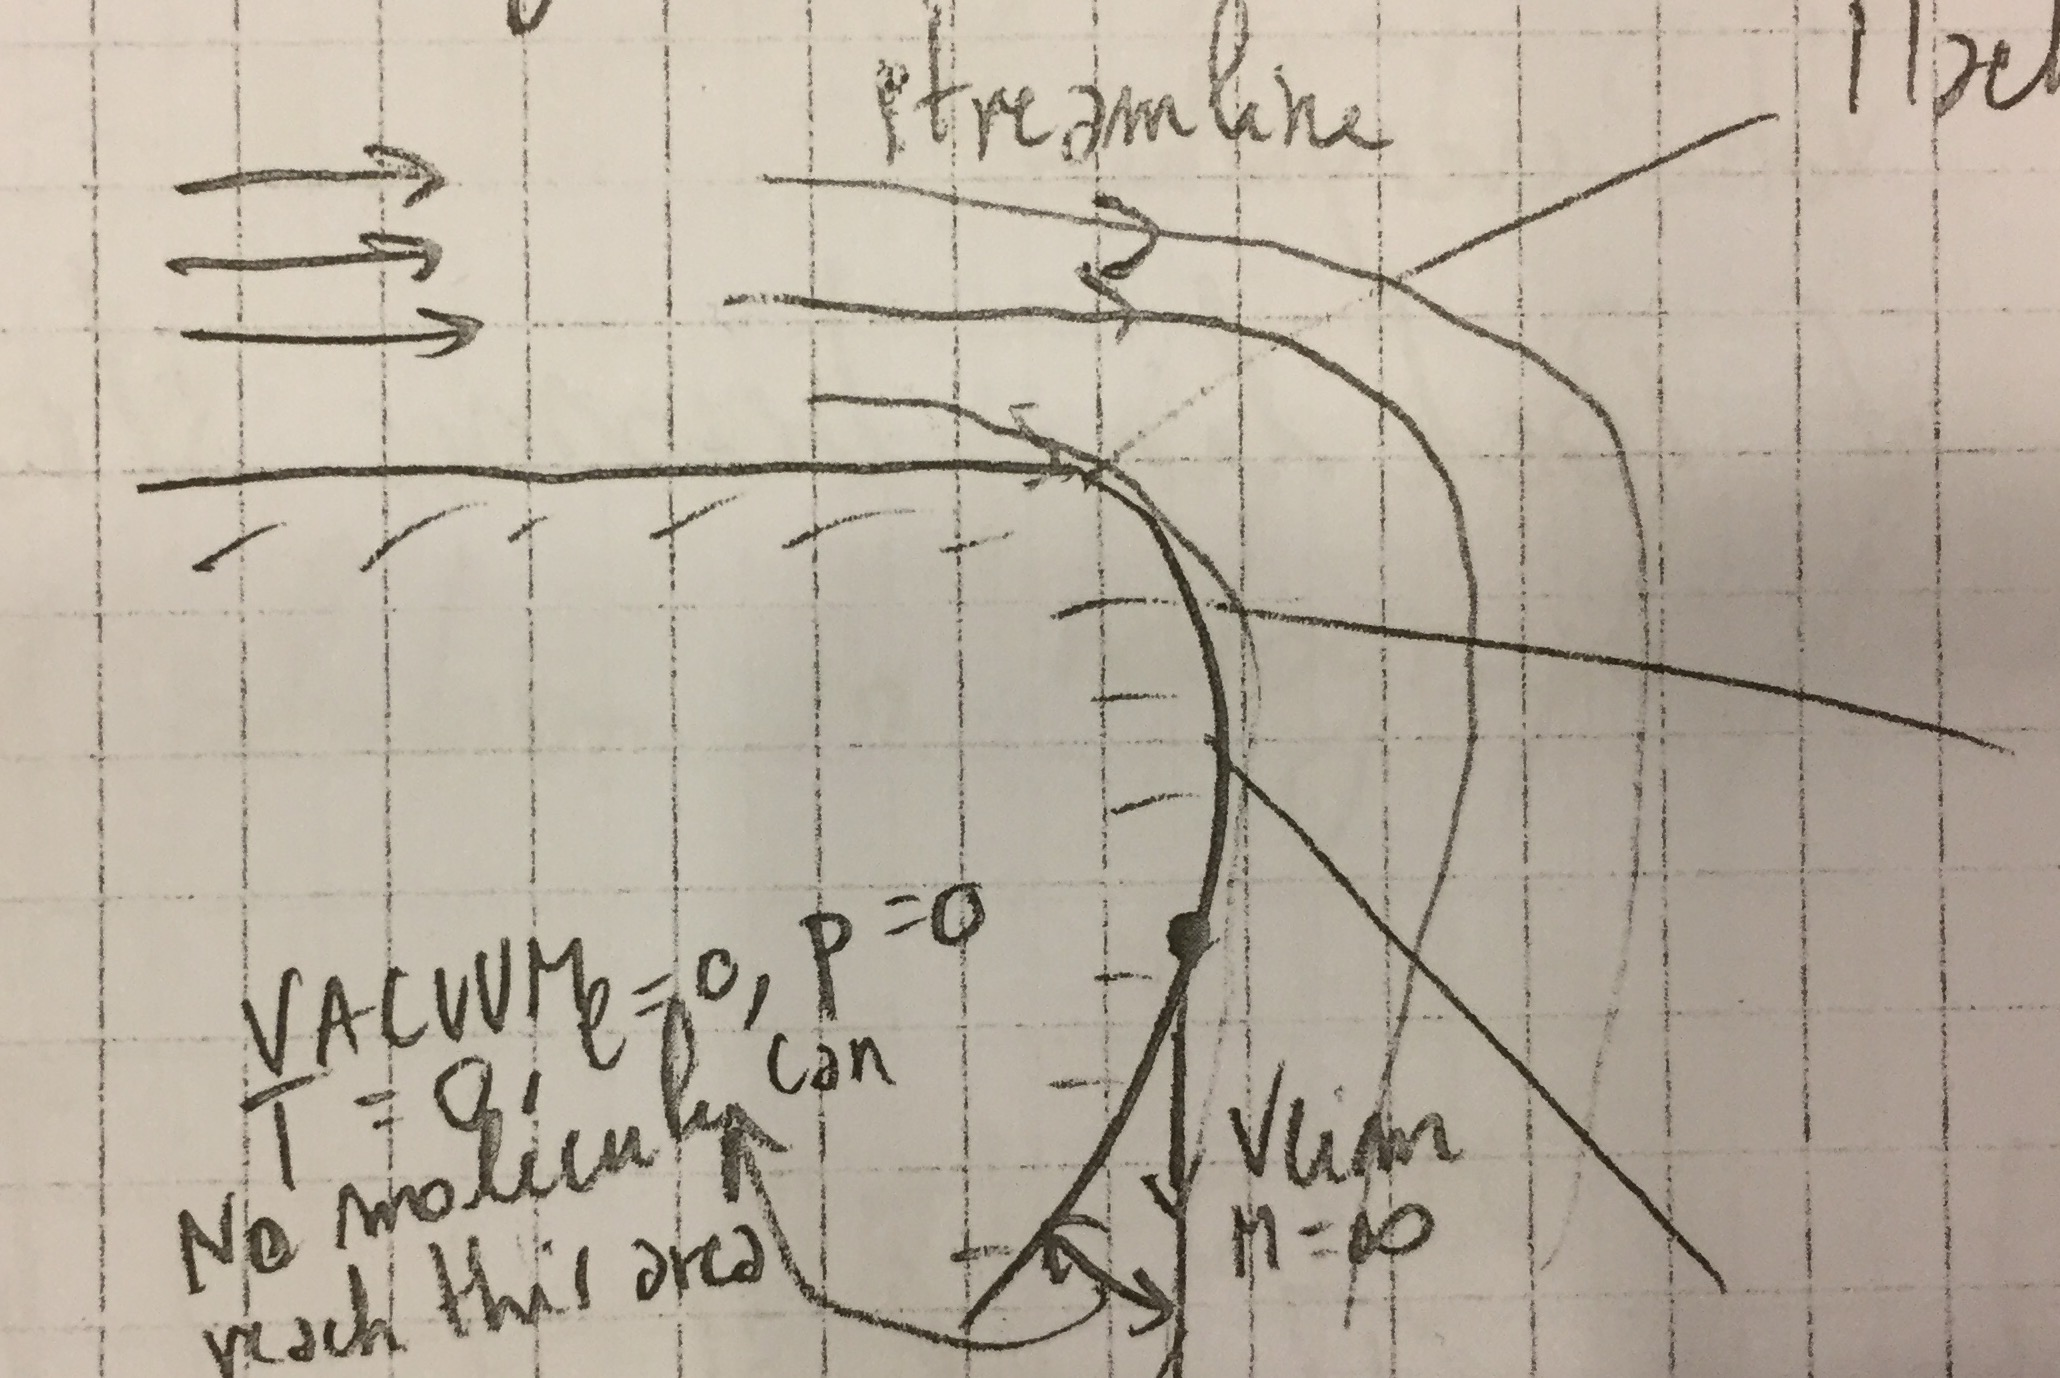
\includegraphics[scale=0.08]{ch8/24}
	\captionof{figure}{}
	\label{ch8/24}
	\end{center}
	
\subsection{Expansion waves}
	\wrapfig{7}{l}{6}{0.15}{ch8/6}{ch8/6}
	Consider in the figure the convention $d\theta < 0$. The infinitely small $d\theta$ induces an infinitely small perturbation noted $V+dV$. Since the Mach wave is also a solution of the flow equations, $V_t$ before and after the Mach wave is the same. We have: 
	
	\ \\
	
	\begin{equation}
	V_t = V\cos \mu = (V+dV) \cos (\mu - d\theta) \qquad \Leftrightarrow 1+\frac{dV}{V} = \frac{\cos \mu }{\cos (\mu - d\theta)}
	\label{eq:8.63}
	\end{equation}
	
	Using the fact that $d\theta$ is very small we get: 
	
	\begin{equation}
	1+\frac{dV}{V} \approx \frac{\cos \mu }{\cos \mu + d\theta \sin \mu } = \frac{1}{1 + d\theta \tan \mu} \approx 1- d\theta \tan \mu \quad \Rightarrow d\theta = - \sqrt{M^2 - 1} \frac{dV}{V} 
	\label{eq:dV/V}
	\end{equation}
	
	Let's now try to rewrite the $dV/V$ as a function of $M$. We know from the definition of M that: 
	
	\begin{equation}
	M = \frac{V}{a} \qquad \Rightarrow \frac{dM}{M} = \frac{dV}{V} - \frac{da}{a}
	\end{equation}
	
	In addition we have the total temperature constant across the shock and its derivative gives: 
	
	\begin{equation}
	\begin{array}{c}
	\gamma R T_t = a^2 \left( 1+ \frac{\gamma -1}{2} M^2\right) = cst \qquad \Leftrightarrow 2ada \left( 1+ \frac{\gamma -1}{2} M^2\right)+ a^2 (\gamma -1) M dM = 0  \\
	\Rightarrow \frac{da}{a} = - \frac{\gamma-1}{2}\frac{MdM}{1+ \frac{\gamma -1}{2} M^2}
	\end{array}
	\end{equation}
	
	We can now replace these values in \eqref{eq:dV/V} and get: 
	
	\begin{equation}
	d\theta = -\frac{\sqrt{M^2 -1}}{1+\frac{\gamma -1}{2} M^2}\frac{dM}{M}
	\end{equation}
	
	and after integration: 
	
	\begin{center}
	\theor{
	\textbf{Prandtl-Meyer function}	
	\begin{equation}
	\theta = - \nu (M) + K^- \qquad \nu (M) = \sqrt{\frac{\gamma + 1 }{\gamma -1}} \arctan \sqrt{\frac{\gamma - 1 }{\gamma +1} (M^2 - 1)} - \arctan\sqrt{M^2 - 1}
	\end{equation}
	}
	\end{center}
	
	Additionally, consider a decrease of $\theta$ between a point 1 and 2, the integration will give: 
	
	\begin{equation}
	\theta _2 - \theta _1 = \delta \theta = -\nu (M_2) + \nu (M_1)
	\end{equation}
	
	Since $\delta \theta < 0$, same for right hand side, meaning $\nu (M_2)>\nu (M_1)$ and since $\nu$ is monotonously increasing with M, $M_2 > M_1 \Rightarrow$ \textbf{expansion}. If the properties in 1 are known, we can find the $\nu (M_2)$ and thus the $M_2$. 
	
	\subsubsection{Reverse case}
	
	\wrapfig{7}{l}{6}{0.12}{ch8/26}{ch8/26}
	In this case $d\theta > 0$ and $\mu < 0$. \autoref{eq:8.63} is still valid and since $d\theta > 0$: 
	
	\begin{equation}
	d\theta = \sqrt{M^2-1}\frac{dV}{V} \qquad \Rightarrow d\theta = \frac{\sqrt{M^2 -1}}{1+\frac{\gamma -1}{2} M^2}\frac{dM}{M}
	\end{equation}
	
	We see that this is the above equations with contrary sign and the angle relation after integration is: 
	
	\begin{equation}
	\theta _2 - \theta _1 = \delta \theta = \nu (M_2) - \nu (M_1)
	\end{equation}
	
	where $M_2 > M_1$ still as $\delta \theta > 0$. Lastly, remark that the integration of $d\theta$ gives: $\theta = \nu (M) + K^+$ which is the equation for $C^+$ in $M,\theta$-plane. 
	
\subsection{Compression wave}
	\wrapfig{7}{l}{6}{0.12}{ch8/25}{ch8/25}
	The same developements could be done in the case $dV < 0$ and this will correspond to a compression wave. Since the equation is still valid we can write: 
	
	\begin{equation}
	\begin{aligned}
	&V_t = V\cos \mu = (V+dV) \cos (\mu - d\theta) \\
	&d\theta = - \sqrt{M^2 - 1} \frac{dV}{V} \\
	&\theta _2 - \theta _1 = \delta \theta = -\nu (M_2) + \nu (M_1)
	\end{aligned}
	\end{equation}
	
	where we can directly deduce the decrease in velocity. The reverse case could also be done here and the same results will be concluded. We have thus 4 situations to take care. 
	
\section{Prandtl-Meyer expansion}
	\wrapfig{11}{l}{6}{0.1}{ch8/27}{ch8/27}
	Now we can consider a bend. This can be subdivided into infinitely small bendings with each involving a change of angle and a Mach wave. As we've seen in last chapters, the Mach wave will keep growing with the angle changes, inducing the Mach wave to decrease continuously, thus the Mach waves never cross each other. When the flow goes through a Mach wave, this induces an infinitely small change of angle, and this done infinitely will end up to a finite change of angle. Remark that the flow in a beginning corner and ending corner is the same.  Again, with this reasoning we can conclude that at a straight corner there are infinite Mach waves in a single point. 
	
	\wrapfig{9}{r}{4}{0.15}{ch8/28}{ch8/28}
	The variation of M is dictated by the $C^-$ curve. The Mach wave is perpendicular to the tangent at the curve at this point. Such flow is called Prandtl-Meyer expansion. 
	
\section{Oblique shock waves}
\subsection{Formation of an oblique shock wave}
	\minifig{ch8/29}{ch8/30}{0.15}{0.15}{0.35}{0.35}
	Consider a supersonic flow over the represented bend, as previously we can infinitely subdivide the bend. Since the flow is deviated at each point, there is a Mach wave at each point and since we have compression waves, the Mach number is decreasing and the slope is increasing at each deviation. It is physically impossible that Mach waves meet, thus we get a shock wave. It is also a solution of the flow equations. 
	
	\wrapfig{5}{l}{4}{0.15}{ch8/31}{ch8/31}
	Similar situation is observed at a corner (the Mach lines intersect directly) and what we observe is an \textbf{oblique shock wave} instead of Mach wave. The angle $\beta \neq \mu $ and has to be determined. Through this, the flow will deviate from a finite angle. The flow equations will be manipulated now. 
	\newpage
\subsection{The characteristic Mach number}
	It is defined as: 
	
	\begin{equation}
	M^* = \frac{q}{a^*} \qquad a^* = \sqrt{\gamma R T^*}
	\end{equation}
	
	where q is the module of the velocity, $a^*$ and $T^*$ the speed of sound and the static temperature at $M=1$. Remind that $T = T_t - \frac{v^2}{2c_p}$, if we use: 
	
	\begin{equation}
	\begin{aligned}
	T_t = T \left(1+ \frac{\gamma - 1}{2}M^2 \right) \qquad &\Rightarrow \left( \frac{M^*}{M}\right)^2 = \frac{T^*}{T} \cdot \left( \frac{T_t}{T_t}\right) = \frac{\frac{\gamma + 1}{2}}{1+ \frac{\gamma -1}{2}M^2}\\
	&\Rightarrow M^{*^2} =  \frac{\frac{\gamma + 1}{2}M^2}{1+ \frac{\gamma -1}{2}M^2}
	\end{aligned}
	\label{eq:8.74}
	\end{equation}
	
	This implicity assumes that the total temperature is conserved across the shock, but this is indeed the case. We directly deduce that: 
	
	\begin{equation}
	M < 1 \Leftrightarrow M^* <1 \qquad M \geq 1 \Leftrightarrow M^* \geq 1
	\label{eq:8.75}
	\end{equation}
	
	Similarly we can define the characteristic normal Mach number: 
	
	\begin{equation}
	M^*_n = \frac{u_n }{a^{**}} \qquad a^{**}  = \sqrt{\gamma R T^{**}}
	\end{equation}
	
	where $a^{**}$ and $T^{**}$ are the speed of sound and static temperature when the normal Mach number = 1. We can express a relation for the temperatures in normal variables from the definition of total temperature: 
	
	\begin{equation}
	\begin{aligned}
	&T_t = T + \frac{\vec{v}^2}{2c_p} \Leftrightarrow T_t - \frac{v_t^2}{2c_p} = T + \frac{v_n^2}{2c_p}\qquad \Leftrightarrow \bar{T}_t = T\left(1 + \frac{\gamma -1}{2}M^2_n \right)\\
	&\Rightarrow T^{**}= \frac{\bar{T}_t}{\frac{\gamma +1}{2}}\qquad \Rightarrow M^{*^2}_n = \frac{\frac{\gamma +1}{2}M^2_n}{1+ \frac{\gamma -1}{2}M^2}
	\end{aligned}
	\end{equation}
	
	We find exactly the same relations as previously and \eqref{eq:8.75} is valid for normal variables. 
	
\subsection{Relations between conditions before and after the shock wave}
\subsubsection{Relation between Mach number before and after the shock}
	\wrapfig{8}{l}{5}{0.15}{ch8/32}{ch8/32}
	Consider a compression with deflection angle $\theta$ leading to the shock wave angle $\beta$. The governing equations are: 
	
	\begin{equation}
	\begin{array}{cc}
	\rho _1 v_{n1} = \rho _2 v_{n2} & p_1 + \rho _1 v_{n1}^2 = p_2 + \rho _2 v_{n2}^2\\
	v_{t1} = v_{t2} & H_1 = H_2\\
	\end{array}
	\end{equation}
	
	If we devide the equation with pressure by $\rho v_n$: 
	
	\begin{equation}
	R\left( \frac{T_1}{v_{n1}} - \frac{T_2}{v_{n2}} \right) = v_{n2} - v_{n1}
	\end{equation}
	
	If we use the constant total temperature across the shock, we find: 
	
	\begin{equation}
	\begin{array}{c}
	\bar{T}_t = T_1 \frac{v_{n1}^2}{2c_p} = T_2 \frac{v_{n2}^2}{2c_p} \qquad \Rightarrow R\left( \frac{T_1}{v_{n1}} - \frac{T_2}{v_{n2}} \right) - \frac{R}{2c_p}\left( v_{n1} - v_{n2} \right) = v_{n2} - v_{n1} \\
	\Rightarrow v_{1n}v_{2n} = \frac{2\gamma }{\gamma +1 } R\bar{T}_t = (a^{**})^2
	\end{array}
	\label{eq:8.80}
	\end{equation}
	
	From this developpement we finally get an important relation for the Mach numbers before and after the shock: 
	
	\begin{center}
	\theor{
	\begin{equation}
	M_{1n}^* M_{2n}^* = 1
\end{equation}		
	}
	\end{center}
	
	We are now able to compute $M_2$ knowing $M_1$. First compute $M_{1n} = M_1 \sin \beta $, then $M_1^*$ using \eqref{eq:8.74}, we get $M_2^*$ from our last relation and we go backward: $M_2 = \frac{M_{n2}}{\sin (\beta -\theta)}$.
	
	\paragraph{Remark} \quad In theory there are two possible cases: 
	
	\begin{equation}
	\begin{aligned}
	&M_{n1} > 1 \Rightarrow M_{n1}^* > 1 \Rightarrow M_{n2}^* < 1 \Rightarrow M_{n2} < 1\\
	 &M_{n1} < 1 \Rightarrow M_{n1}^* < 1 \Rightarrow M_{n2}^* > 1 \Rightarrow M_{n2} > 1
	\end{aligned}
	\end{equation}
	
	The second one corresponds to an expansion wave and is physically not possible because it leads to an decrease of entropy as we will see later. 
	
\subsubsection{Relation between the density before and after the shock}
	From the mass conservation equation we directly get:
	
	\begin{center}
	\theor{
	\begin{equation}
	\frac{\rho _2}{\rho _1} = \frac{v_{n1}}{v_{n2}} \left(\frac{v_{n1}}{v_{n1}} \right) = \frac{v_{n1}^2}{a^{**^2}} = M^{*^2}_{n1}
	\end{equation}
	}
	\end{center}
	and we conclude that the density over the shock increases. 
	
\subsubsection{Relation between pressure before and after the shock}
	We begin from the equation with pressures: 
	
	\begin{equation}
	\frac{p_2}{p_1} = 1 + \frac{\rho _1v_{n1}^2}{p_1} - \frac{\rho _2v_{n2}^2}{p_1} = 1 + \frac{\rho _1v_{n1}}{p_1}\left( 1 - \frac{v_{n2}}{v_{n1}} \left( \frac{v_{n1}}{v_{n1}}\right)\right) 
	\end{equation}
	
	where if we use \eqref{eq:8.80} and \eqref{eq:8.74} we find that 
	
	\begin{center}
	\theor{
	\begin{equation}
	\frac{p_2}{p_1}=	1+ \frac{2\gamma }{\gamma +1} (M^2_{n1} - 1)
\end{equation}		
	}
	\end{center}
	
\subsubsection{Entropy variation over the shock}
	We begin from the general entropy definition and apply the perfect gas relation: 
	
	\begin{equation}
	T ds = dh - \frac{dp}{\rho} \Leftrightarrow ds = c_p \frac{dT}{T} - R\frac{dp}{p}
	\end{equation}
	
	We can now switch to the total variables since this transformation is always isentropic, and since the total temperature is constant we have: 
	
	\begin{center}
	\theor{
	\begin{equation}
	ds = - R \frac{dp_t }{p_t} \qquad \Rightarrow s_2 - s_1 = -R\ln \left( \frac{p_{t2}}{p_{t1}}\right)
	\end{equation}
	}
	\end{center}
	
	Since $s_2>s_1$ must be satisfied, we must have $p_{t2}<p_{t1}$ and we have thus a loss of total pressure. To determine it, let's begin from the valid relation:
	
	\begin{equation}
	\frac{p_t}{p} = \left(\frac{T_t}{T} \right)^{\frac{\gamma}{\gamma -1}} \qquad \Rightarrow \frac{p_{t2}}{p_{t1}} = \frac{p_2}{p_1}\left(\frac{T_1}{T_2} \right)^{\frac{\gamma}{\gamma -1}} = \left(\frac{p_1}{p_2} \right)^{\frac{1}{\gamma -1}}\left(\frac{\rho _2}{\rho _1} \right)^{\frac{\gamma}{\gamma -1}}
	\end{equation}
	
\subsubsection{Relation between variation of $\bm{\rho}$ and p over the shock}
	\wrapfig{6}{l}{6}{0.15}{ch8/33}{ch8/33}	
	We can now determine all the variables from $M_1$. Combination of pressure relation and density relation gives the: 
	
	\ \\\\\\\\\\
	
	\begin{center}
	\theor{
	\textbf{Rankine-Hugoniot}
	\begin{equation}
	\frac{\rho _2}{\rho _1} = \frac{\frac{\gamma +1}{\gamma -1} + \frac{p_1}{p_2}}{1 + \frac{\gamma +1}{\gamma -1} \frac{p_1}{p_2}}
	\end{equation}
	}
	\end{center}
	
	\wrapfig{6}{l}{2}{0.15}{ch8/34}{ch8/34}	
	Note the difference with the isentropic relation: $\frac{\rho _2 }{\rho _1} = \left(\frac{p_2}{p_1} \right)^{\frac{1}{\gamma}}$. Here is plotted the two curves, one sees clearly that they differ. Above that curve we have expansion and under it is the compression and the curves correspond to $S_2=S_1$. We can also see that for infinitely weak shock waves, the isentropic curve coincide, the shock wave is therefor a Mach wave in the infinitely weak case. 
	
	\ \\\\\\
	
\subsection{Relation between Mach number, deflection angle $\theta$ and shock wave angle $\beta$}
	\wrapfig{6}{l}{5}{0.15}{ch8/35}{ch8/35}	
	Referring to the figure we can note: $\tan \beta = \frac{u_{n1}}{u_{t1}}$ and $\tan (\beta - \theta ) = \frac{u_{n2}}{u_{t2}}$. After further developpements: 
	
	\begin{equation}
	\begin{aligned}
	&\tan (\beta - \theta) = \frac{1}{M^{*2}_{n1}} = \frac{2 + (\gamma -1 )M_1^2\sin ^2 \beta }{(\gamma  +1) M_1^2\sin ^2 \beta}\\
	&\Leftrightarrow \tan \theta = 2 \coth \beta \frac{M_1^2\sin ^2 \beta -1}{M_1^2 (\gamma + \cos 2\beta ) +2}
	\end{aligned}	
	\end{equation}
	
	We find thus a relation between $\theta, \beta$ and $M_1$ and this can be plot on the ($\theta, \beta$) plane.
	
\subsubsection{Interpretation of the $\beta, \theta, M$ curves}
	\minifig{ch8/36}{ch8/37}{0.12}{0.16}{0.49}{0.49}
	For a given $M, \theta$, there are two possible $\beta$. The highest is the \textbf{strong shock} and the lower is the \textbf{weak shock}. This is due to the increasing pressure gradient between regions 2 and 1 when $\beta$ increases. The solution depends on the downstream pressure condition, if we have a low pressure, weak shock is more likely appearing and the contrary when a high pressure is imposed. \textbf{In this course we always take the weak shock!} \\
	
	Now take for example $M=2$ and $\theta = 30\degres$, there is no solution on the graph. In this case there is no straight oblique shock but a \textbf{detached bow shock}, it occurs upstream the corner and is bent.  Note that for higher $M_1$ the $\theta _{max}$ increases and after $46\degres$ there is no attached solution. \\
	
	Now look at $\theta = 0\degres$, one of the solution is $\beta = 90\degres$ whatever $M_1$ and the other solution is dependent on $M_1$. The first case corresponds to a \textbf{normal shock}. The other one corresponds to $\beta = \mu$ and thus the \textbf{Mach wave}, as previously seen this is the infinitely weak solution.
	
	\minifig{ch8/38}{ch8/39}{0.15}{0.15}{0.49}{0.49}
	If we increase the Mach number keeping the deflection constant, we have $\beta$ decreasing, but this means that pressure ratio is increasing. The shock is stronger. When the velocity is kept constant and the deflection increases, $\beta$ increases and this also means that the pressure ratio increases and thus the wave gets stronger. This has an application for supersonic planes that try to get the weakest shock. As the temperature rising is higher for stronger shock, this is to avoid. 
	
\subsubsection{Mach number after an oblique shock}
	\wrapfig{6}{l}{5}{0.12}{ch8/40}{ch8/40}	
	Let's determine if the velocity after the oblique shock is whether increasing or decreasing. For this, we search for the locus of the points on the graph where $M_2 = 2$. We have two equations for this using the previous relations: 
	
	\begin{equation}
	\sin ^2 (\beta - \theta) = \frac{1 + \frac{\gamma -1}{2} M_1^2 \sin ^2 \beta}{-\frac{\gamma - 1}{2}+ \gamma M_1^2 \sin ^2 \beta}\qquad  \tan \theta = 2 \coth \beta \frac{M_1^2\sin ^2 \beta -1}{M_1^2 (\gamma + \cos 2\beta ) +2}
	\end{equation}
	
	Fixing $M_2=1$ and making $M_1$ vary gives the following figure. Above the curve the flow is subsonic and under, supersonic after a shock. This means that for strong shocks and normal shock we have always a subsonic flow. For weak shock it is supersonic, except for deflections close to the maximal value. 
	
\subsection{Application: supersonic inlets of planes}
	\wrapfig{6}{l}{5}{0.12}{ch8/40}{ch8/41}
	The first one is the \textbf{Pitot inlet}, since the engine requires a subsonic flow, a normal detached shock appears upstream the inlet. This leads to a high pressure loss, for example $M=3 \rightarrow \frac{p_{t2}}{p_{t1}} = 0.328$. This ratio is related to the entropy increase and thus the efficiency of the flow, thus the engine. For this reason, they are only used up to $M = 1.6$. 
	
	\ \\
	
	The other case consists in producing an oblique shock before the normal shock. This slows down the flow before the normal shock which is thus weakened. The pressure loss in this case is lower than the previous (see example in course for more details).
	
\section{Conical oblique shock waves}
	The analysis we made is in 2D, remark that there is some changes in the 3D case. First of all, the shape of the shock is not a triangle but conical. Then it is weakened because there is a third direction for the flow to move on. The deflection of the flow after the shock is lower (only 8\degres for 20\degres deflection) and has to bend then to reach the angle. 